\documentclass[border=5pt]{standalone}
\usepackage{tikz}
\usepackage{amsmath}
\usetikzlibrary{arrows.meta,calc,positioning,fit,backgrounds}
\definecolor{cpl}{RGB}{28,90,214}   % coupling blue
\definecolor{gh}{RGB}{110,110,110}  % ghost grey
\tikzset{
  bus/.style={circle, draw, line width=0.7pt, minimum size=15pt, inner sep=0pt, font=\footnotesize},
  ghost/.style={circle, draw=gh, line width=0.7pt, densely dotted, minimum size=15pt, inner sep=0pt, font=\footnotesize, text=gh},
  branch/.style={line width=0.75pt},
  stub/.style={gh, line width=0.75pt, densely dotted},
  halfl/.style={line width=0.75pt},
  zbox/.style={draw, fill=black!9, rounded corners=2pt, inner sep=3pt, font=\footnotesize},
  couple/.style={cpl, densely dotted, line width=0.9pt},
  cplab/.style={font=\scriptsize, text=cpl, inner sep=1.5pt},
  zone/.style={draw, dashed, rounded corners=7pt, line width=0.8pt, inner sep=0pt},
  zlab/.style={font=\scriptsize\itshape, text=black!55},
  gen/.style={circle, draw, line width=0.6pt, minimum size=11pt, inner sep=0pt, font=\scriptsize},
}

\begin{document}
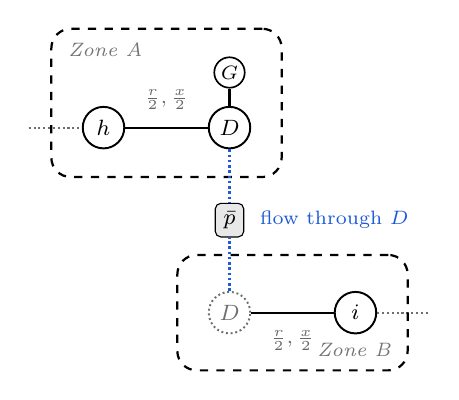
\begin{tikzpicture}
% ---------------- Zone A (top): from-zone, D real + generator ----------------
\node[bus] (hA) at (0.3,2.35) {$h$};
\node[bus] (DA) at (1.9,2.35) {$D$};
\node[gen] (gn) at (1.9,3.05) {$G$};
\draw[branch] (DA) -- (gn);
\draw[stub]   (-0.65,2.35) -- (hA);
\draw[halfl]  (hA) -- (DA);
\node[font=\scriptsize, text=black!60, anchor=south] at (1.1,2.45) {$\tfrac{r}{2},\tfrac{x}{2}$};
\node[zone, fit=(hA)(DA)(gn), inner xsep=11pt, inner ysep=10pt] (zA) {};
\node[zlab, anchor=north west] at ([shift={(3pt,-2pt)}]zA.north west) {Zone A};

% ---------------- Zone B (bottom): to-zone, D ghost ----------------
\node[ghost] (DB) at (1.9,0.0) {$D$};
\node[bus]   (iB) at (3.5,0.0) {$i$};
\draw[halfl]  (DB) -- (iB);
\draw[stub]   (iB) -- (4.45,0.0);
\node[font=\scriptsize, text=black!60, anchor=north] at (2.7,-0.1) {$\tfrac{r}{2},\tfrac{x}{2}$};
\node[zone, fit=(DB)(iB), inner xsep=11pt, inner ysep=13pt] (zB) {};
\node[zlab, anchor=south east] at ([shift={(-3pt,2pt)}]zB.south east) {Zone B};

% ---------------- consensus: flow through D ----------------
\node[zbox] (zp) at (1.9,1.175) {$\bar p$};
\draw[couple] (DA) -- (zp);
\draw[couple] (DB) -- (zp);
\node[cplab, anchor=west] at ([xshift=4pt]zp.east) {flow through $D$};
\end{tikzpicture}
\end{document}
